
% ---
% Configurações
% ---

\documentclass[
	% -- opções da classe memoir --
	article,			% indica que é um artigo acadêmico
	12pt,				% tamanho da fonte
	oneside,			% para impressão apenas no verso. Oposto a twoside
	a4paper,			% tamanho do papel.
	% -- opções da classe abntex2 --
	%chapter=TITLE,		% títulos de capítulos convertidos em letras maiúsculas
	%section=TITLE,		% títulos de seções convertidos em letras maiúsculas
	%subsection=TITLE,	% títulos de subseções convertidos em letras maiúsculas
	%subsubsection=TITLE % títulos de subsubseções convertidos em letras maiúsculas
	% -- opções do pacote babel --
	english,			% idioma adicional para hifenização
	brazil,				% o último idioma é o principal do documento
	sumario=tradicional
	]{abntex2}


% ---
% Pacotes fundamentais
% ---

\usepackage{lmodern}			% Usa a fonte Latin Modern
\usepackage[T1]{fontenc}		% Selecao de codigos de fonte.
\usepackage[utf8]{inputenc}		% Codificacao do documento (conversão automática dos acentos)
\usepackage{indentfirst}		% Indenta o primeiro parágrafo de cada seção.
\usepackage{nomencl} 			% Lista de simbolos
\usepackage{color}				% Controle das cores
\usepackage{graphicx}			% Inclusão de gráficos
\usepackage{microtype} 			% para melhorias de justificação
\usepackage{lipsum}				% para geração de dummy text
\usepackage[brazilian,hyperpageref]{backref}	 % Paginas com as citações na bibl
\usepackage[alf]{abntex2cite}	% Citações padrão ABNT
\usepackage{mathptmx}
\usepackage{appendix}
\usepackage{titling}

% ---
% Elementos pré-textuais
% ---

\titulo{Modelo para elaboração de TCCs na forma de artigo do Curso de Estatística - UFPR }


\autor{Alexandre Morales Diaz \and
Simone Matsubara \and
Willian Meira Schlichta}

\thanksmarkseries{arabic}
\date{}

\makeindex

% ---
% Configuração de margens, espaçamentos entre linhas e parágrafos
% ---

\setlrmarginsandblock{2.5cm}{2.5cm}{*}
\setulmarginsandblock{2.5cm}{2.5cm}{*}
\checkandfixthelayout
% ---
% O tamanho do parágrafo é dado por:
\setlength{\parindent}{1.3cm}

% Controle do espaçamento entre um parágrafo e outro:
\setlength{\parskip}{0.2cm}  % tente também \onelineskip

% Espaçamento simples
\SingleSpacing

% ----
% Início do documento
% ----

\begin{document}

% Retira espaço extra obsoleto entre as frases.
\frenchspacing


% ---
% Resumo
% ---

\maketitle
\vspace{-1cm}
% resumo em português
\begin{resumoumacoluna}
 Relatório de análise do o artigo Análise Comparativa de Modelos Para Dados Longitudinais no Estudo da Contagem do Número de Bactérias
 Presentes no Leite de Vaca 
       
       realizado como parte da avaliação da disciplina da Análise de Dados Longitudinais
 
 
 
 Conforme a ABNT NBR 6022:2003, o resumo é elemento obrigatório, constituído de
 uma sequência de frases concisas e objetivas e não de uma simples enumeração
 de tópicos, não ultrapassando 250 palavras, seguido, logo abaixo, das palavras
 representativas do conteúdo do trabalho, isto é, palavras-chave e/ou
 descritores, conforme a NBR 6028. (\ldots) As palavras-chave devem figurar logo
 abaixo do resumo, antecedidas da expressão Palavras-chave: separadas entre si por
 ponto e finalizadas também por ponto. Evitar repetir termos que já aparecem no título do trabalho. Usar 4 a 6 palavras chaves.

 \vspace{\onelineskip}

 % ---
% Palavras-chaves
% ---

 \noindent
 \textbf{Palavras-chave}: Estatística. Latex. Normas técnicas. Trabalho acadêmico.
\end{resumoumacoluna}

% ]  				

% ----------------------------------------------------------
% Elementos textuais
% ----------------------------------------------------------
\textual

% ----------------------------------------------------------
% Introdução
% ----------------------------------------------------------
\section{Introdução}

Adicionar o conteúdo da introdução. Exemplos de citação: \citeonline{chatterjee2009distribution} afirmam que a>b. No entanto, c<d \cite{park2009median}. As seções seguintes devem apresentar a revisão de literatura, metodologia do trabalho, resultados e discussão. Os títulos das seções (e das sub-seções), no entanto, ficam a critério dos autores. Recomenda-se que a última seção seja intitulada "Considerações finais". As referências bibliográficas são obrigatórias.



% ----------------------------------------------------------
% Seções
% ----------------------------------------------------------

\section{Modelos lineares generalizados}
Bla bla bla bla bla bla bla bla bla bla bla bla bla bla bla bla bla bla bla bla bla bla bla bla bla bla bla bla bla bla bla bla bla bla bla bla bla bla bla bla bla bla bla bla bla bla bla bla bla bla bla bla bla bla bla bla bla bla bla bla bla bla bla bla bla bla bla bla bla bla bla

Exemplo de como incluir uma figura e uma tabela:

\begin{figure}[ht]
    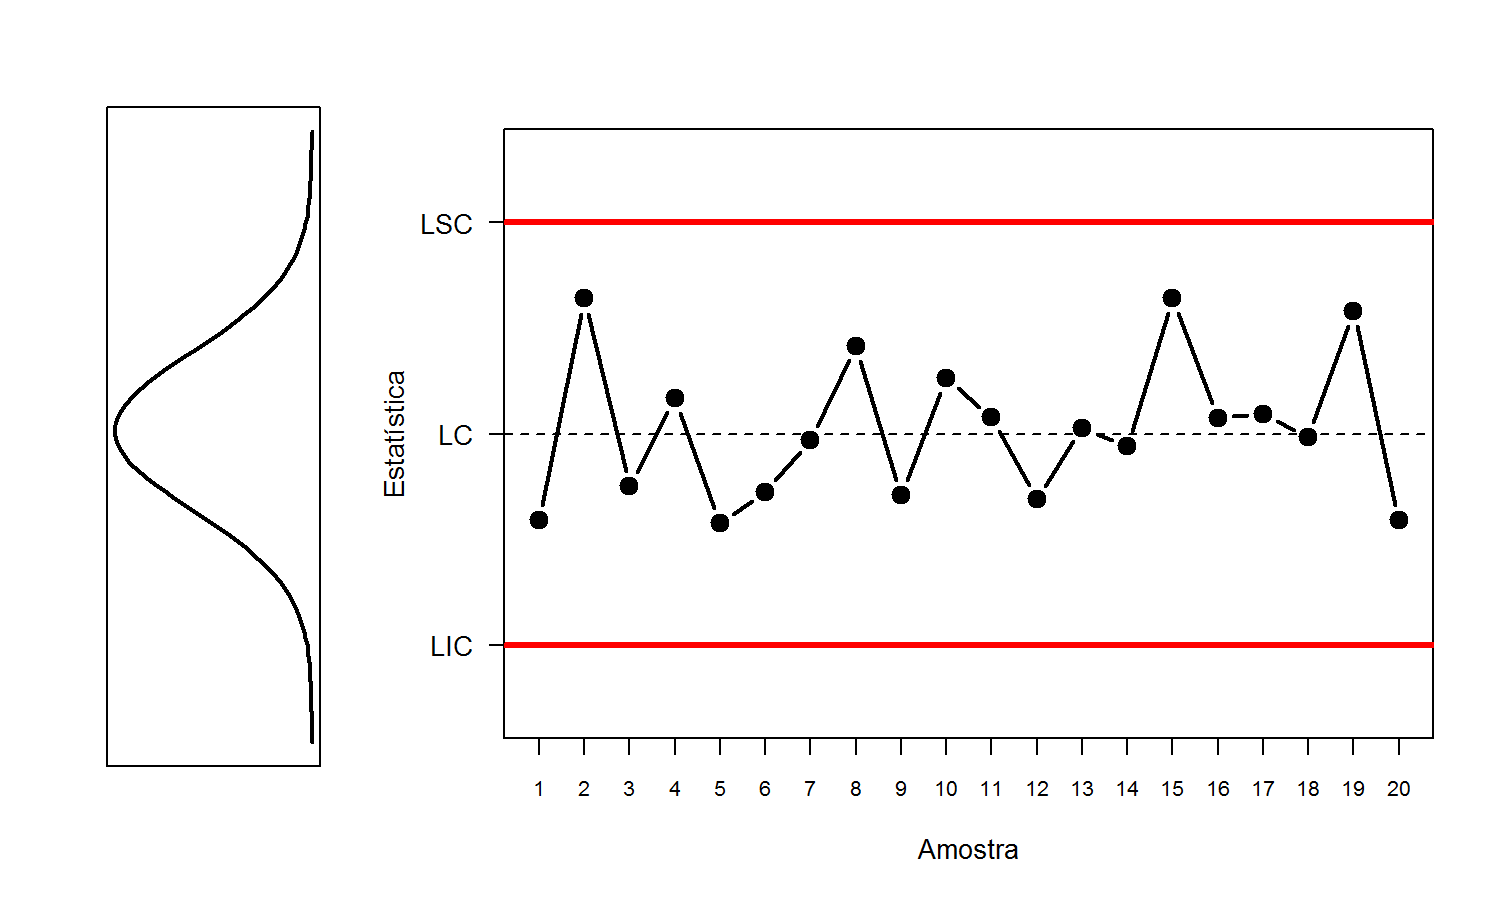
\includegraphics[scale=0.70]{GrafControle.png}
    \caption{Ilustração de um gráfico de controle}
    \label{Fig1}
    \centering
\end{figure}

\begin{table}[]
\center
\caption{Exemplo de tabela}
\begin{tabular}{cccc}
\hline
Fator 1 & Fator 2 & Dose & Resposta \\ \hline
A & C & 5 & 20 \\
A & D & 5 & 18 \\
B & C & 5 & 12 \\
B & D & 5 & 15 \\ \hline
\end{tabular}
\end{table}

\subsection{Modelos lineares generalizados para dados de contagens}
Bla bla bla bla bla bla bla bla bla bla bla bla bla bla bla bla bla bla bla bla bla bla bla bla bla bla bla bla bla bla bla bla bla bla bla bla bla bla bla bla bla bla bla bla bla bla bla bla bla bla bla bla bla bla bla bla bla bla bla bla bla bla bla bla bla bla bla bla bla bla bla

\subsection{Modelos de quase verossimilhança}
Bla bla bla bla bla bla bla bla bla bla bla bla bla bla bla bla bla bla bla bla bla bla bla bla bla bla bla bla bla bla bla bla bla bla bla bla bla bla bla bla bla bla bla bla bla bla bla bla bla bla bla bla bla bla bla bla bla bla bla bla bla bla bla bla bla bla bla bla bla bla bla

\subsection{Super dispersão e excesso de zeros}
Bla bla bla bla bla bla bla bla bla bla bla bla bla bla bla bla bla bla bla bla bla bla bla bla bla bla bla bla bla bla bla bla bla bla bla bla bla bla bla bla bla bla bla bla bla bla bla bla bla bla bla bla bla bla bla bla bla bla bla bla bla bla bla bla bla bla bla bla bla bla bla

\section{Estudo de simulação}
Bla bla bla bla bla bla bla bla bla bla bla bla bla bla bla bla bla bla bla bla bla bla bla bla bla bla bla bla bla bla bla bla bla bla bla bla bla bla bla bla bla bla bla bla bla bla bla bla bla bla bla bla bla bla bla bla bla bla bla bla bla bla bla bla bla bla bla bla bla bla bla

\section{Aplicação em dados reais}
Bla bla bla bla bla bla bla bla bla bla bla bla bla bla bla bla bla bla bla bla bla bla bla bla bla bla bla bla bla bla bla bla bla bla bla bla bla bla bla bla bla bla bla bla bla bla bla bla bla bla bla bla bla bla bla bla bla bla bla bla bla bla bla bla bla bla bla bla bla bla bla

\section{Considerações finais}
Bla bla bla bla bla bla bla bla bla bla bla bla bla bla bla bla bla bla bla bla bla bla bla bla bla bla bla bla bla bla bla bla bla bla bla bla bla bla bla bla bla bla bla bla bla bla bla bla bla bla bla bla bla bla bla bla bla bla bla bla bla bla bla bla bla bla bla bla bla bla bla

% ----------------------------------------------------------
% Referências bibliográficas
% ----------------------------------------------------------

\vspace{1cm}
\bibliography{referencias}

% ----------------------------------------------------------
% Apêndices
% ----------------------------------------------------------

\vspace{1cm}

\appendix
\chapter{APÊNDICES}

\section{Notações}
Bla bla bla bla bla bla bla bla bla bla bla bla bla bla bla bla bla bla bla bla bla bla bla bla bla bla bla bla bla bla bla bla bla bla bla bla bla bla bla bla bla bla bla bla bla bla bla bla bla bla bla bla bla bla bla bla bla bla bla bla bla bla bla bla bla bla bla bla bla bla bla

\section{Resultados complementares}
Bla bla bla bla bla bla bla bla bla bla bla bla bla bla bla bla bla bla bla bla bla bla bla bla bla bla bla bla bla bla bla bla bla bla bla bla bla bla bla bla bla bla bla bla bla bla bla bla bla bla bla bla bla bla bla bla bla bla bla bla bla bla bla bla bla bla bla bla bla bla bla


\end{document} 